\documentclass[11pt,a4paper]{article}
\usepackage[margin=2.3cm]{geometry}
\usepackage{fontspec}
\usepackage{graphicx}
\usepackage{caption}
\captionsetup{font=small,labelfont=bf,skip=4pt,hypcap=false}
\usepackage{amsmath,amssymb,booktabs}
\usepackage{xcolor}
\usepackage[colorlinks=true,allcolors=blue!45!black]{hyperref}
\setlength{\parindent}{1em}
\setlength{\parskip}{4pt}
\newcommand{\ext}{\mathrm{ext}}
\newcommand{\GB}{\mathrm{GB}}
\newcommand{\dd}{\mathrm{d}}
\newcommand{\arxiv}[1]{\href{https://arxiv.org/abs/#1}{arXiv:#1}}
\begin{document}
\begin{center}
{\Large\bfseries Rotating black holes at finite\par Gauss--Bonnet coupling}\\[7pt]
{\large What was done, what was found, and what remains open}\\[5pt]
{\small A summary of the \texttt{BHs} project · 28 September 2026}
\end{center}

\noindent The question behind this work is concrete: at fixed black hole angular momenta, how does the mass of the extremal branch change when a Gauss--Bonnet correction is added to Einstein gravity? Numerical solutions were constructed in five dimensions, their response to the coupling was computed, and that response was extrapolated to zero temperature. The data indicate a positive slope that first decreases and then recovers. The extremal mass keeps increasing; it is the rate of that increase that varies non-monotonically.

\section*{1. The physical problem and the scope of the contribution}
The theory under study has action
\begin{equation}
 I=\frac{1}{16\pi G}\int\dd^5x\sqrt{-g}\,[R+\alpha\mathcal L_{\GB}],
 \qquad \mathcal L_{\GB}=R^2-4R_{ab}R^{ab}+R_{abcd}R^{abcd}.
\end{equation}
The solutions are stationary and asymptotically flat, with a spherical horizon and two equal angular momenta, $J_1=J_2=J$. This equality reduces the problem to radial functions. Throughout, $G=1$ and $J$ denotes the angular momentum in each plane. Varying $\alpha$ means comparing solutions of different theories, rather than evolving a coupling within a single spacetime.

The starting point is known. At zero coupling one recovers Myers--Perry; at first order, the result published by Ma, Li and Lü~\cite{pert} is
\begin{equation}
 M_\ext(J,\alpha)=\frac32\pi^{1/3}J^{2/3}+\pi\alpha+O(\alpha^2).
 \label{eq:pert}
\end{equation}
The initial slope is therefore $\pi$. This formula serves as an external reference, not as a new result of the project. The aim is to measure how much that slope changes once the coupling is no longer infinitesimal.

The existence of these solutions is also established: Brihaye and collaborators constructed rotating families at finite coupling, and Kleihaus, Kunz and Radu studied their extremal branch directly~\cite{egb}. Their domain of existence already contains information about the extremal mass. The contribution sought here is more specific: to obtain its derivative with respect to $\alpha$ as a local thermodynamic response, resolve its coupling dependence, and relate it to the behaviour of non-extremal states.

This distinction matters when interpreting the result. The project follows the branch connected to Myers--Perry. It does not establish uniqueness, stability, or a minimum mass among all possible geometries with the same angular momenta. Nor does it study gravitational waves or mergers: this is an equilibrium calculation. The references on higher dimensions and numerical methods provide the framework~\cite{er,dsw}; corrections to extremal Kerr motivate caution about the zero-temperature limit~\cite{h}, but their conclusions do not automatically carry over to this theory.

\newpage
\section*{2. From the equations to a family of solutions}
The development began with Myers--Perry in vacuum and Boulware--Deser in the static sector: their known solutions provided checks of the geometries, charges, and horizon conditions. For the rotating family, the radial equations for $b,f,h,w$ and their regular expansions were derived. The constraint and tensor evaluations away from the nodes provide checks beyond the solver residual.

The exterior is compactified and discretised on Chebyshev--Lobatto nodes. A damped Newton method solves the equations at fixed $(r_H,\Omega_H,\alpha)$, and continuation uses each accepted solution as the seed for the next. Charges are extracted at infinity; temperature and entropy, at the horizon. The production dataset contains \textbf{356 states at 13 couplings}, with base resolution $N=64$ and refinement for difficult states.

\begin{center}
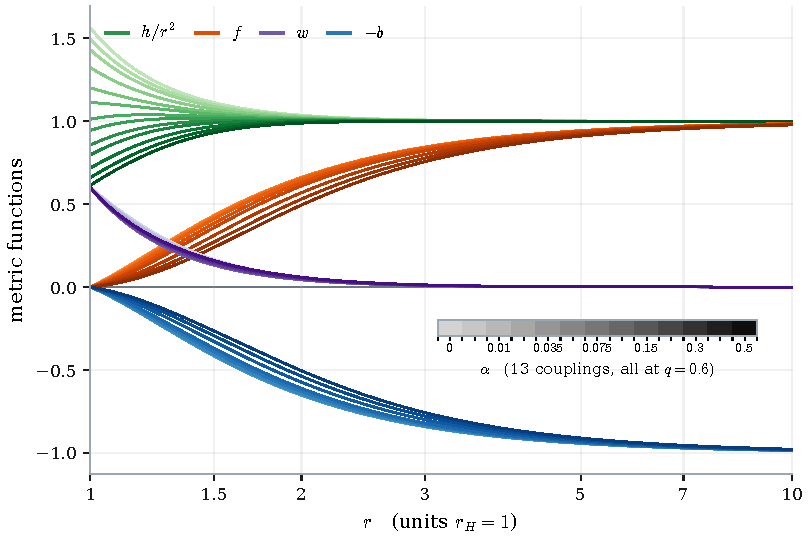
\includegraphics[width=.90\textwidth]{figures/fig-profiles.pdf}
\captionof{figure}{Profiles of the rotating family at 13 values of $\alpha$ between $0$ and $0.5$, with $q=\Omega_Hr_H=0.6$ and $r_H=1$. Each colour identifies a function; darker shades indicate larger coupling. The plot shows $f$, $-b$, $h/r^2$ and $w$ against $r$ on a logarithmic axis. These conventions separate $b$ from $f$ and remove the asymptotic growth of $h$.}
\label{fig:profiles}
\end{center}

Shooting, radial integration, adaptive methods, and neural seeds were also explored. The adaptive comparisons shared spectral seeds, which limits their independence. The network only proposed initial approximations: acceptance still required solving the equations and passing the physical checks. Failed attempts were retained; a failure to converge was not interpreted as a physical boundary of the family.

\newpage
\section*{3. The quantity that measures the shift}
The central tool is the potential conjugate to Gauss--Bonnet coupling,
\begin{equation}
 \dd M=T\dd S+2\Omega_H\dd J+\Psi\dd\alpha,
 \qquad \Psi=\left(\frac{\partial M}{\partial\alpha}\right)_{S,J}.
 \label{eq:firstlaw}
\end{equation}
The factor of two counts the two rotation planes. The potential is a number associated with each solution: it measures the mass variation due to the change of theory after subtracting the contributions from changes in entropy and angular momentum. The calculation uses Wald entropy, including the curvature correction to the area term.

The solver fixes $r_H$ and $\Omega_H$, rather than $S$ and $J$. The first law allows this path to be used without confusing the constraints:
\begin{equation}
 \boxed{\Psi=M_\alpha-T S_\alpha-2\Omega_H J_\alpha,}
 \qquad \text{derivatives at fixed }(r_H,\Omega_H).
 \label{eq:response}
\end{equation}
The subtraction is essential. In the static limit, the known formulas give $M_\alpha|_{r_H}=3\pi/4$, but subtracting $T S_\alpha$ yields
\begin{equation}
 \Psi_{\mathrm{static}}=\frac{3\pi}{4}\frac{4\alpha-3r_H^2}{r_H^2+4\alpha}.
\end{equation}
At zero coupling this is $-9\pi/4$: the mass increases at fixed radius but decreases at fixed entropy. With rotation, one also subtracts $2\Omega_HJ_\alpha$.

The derivatives are computed by implicitly differentiating the discrete problem,
\begin{equation}
 R_N(u;\alpha,r_H,\Omega_H)=0,
 \qquad
 A u_\alpha=-R_{N,\alpha},\qquad A=\frac{\partial R_N}{\partial u}.
\end{equation}
A linear solve gives the profile response; the chain rule gives the responses of $M,J,S$, including the explicit dependence of entropy on $\alpha$. Local derivatives are evaluated by complex step. This avoids subtracting masses of solutions at neighbouring couplings, but does not eliminate discretisation error, conditioning effects, or roundoff. The implicit identity is exact for a differentiable branch of the discrete system; its evaluation remains numerical.

Finally, along a regular extremal branch at fixed $J$,
\begin{equation}
 \left(\frac{\partial M_\ext}{\partial\alpha}\right)_J=\Psi_\ext,
 \qquad
 \left(\frac{\partial S}{\partial\alpha}\right)_{M,J}=-\frac{\Psi}{T}\quad(T>0).
\end{equation}
The first equality requires the entropy term in the first law to vanish in the limit. The second expresses the sign relation between entropy and extremality~\cite{gp}. These consequences were derived and checked algebraically in the project; the extended first law and entropy formula are taken from the literature. They imply no claim about the weak gravity conjecture for this electrically uncharged system.

The checks recover the static and Einstein limits, the perturbative potential, and the extremal entropy from the near-horizon geometry. In the records, Smarr reproduces $\Psi$ with a maximum relative deviation of $1.45\times10^{-6}$ over 313 states; a curvature integral gives $4.67\times10^{-7}$ over 43 profiles. Both routes share the underlying solutions. The sign change of $\Psi$ away from extremality was also mapped, and the valley in $\Psi_\ext$ was related to a maximum of $\Omega_HJ^{1/3}$.

\newpage
\section*{4. The potential and the extremal mass}
States with $T>0$ are extrapolated using a cubic fit to the six coldest; exactly extremal solutions are not constructed. The bands compare 21 fitting variants and express sensitivities, not confidence intervals. The figures use $y=\alpha/J^{2/3}$ and $\mu=M_\ext/J^{2/3}$: at fixed $J$, their axes represent coupling and mass in constant units, with $\Psi_\ext=\mu'(y)$.

\begin{center}
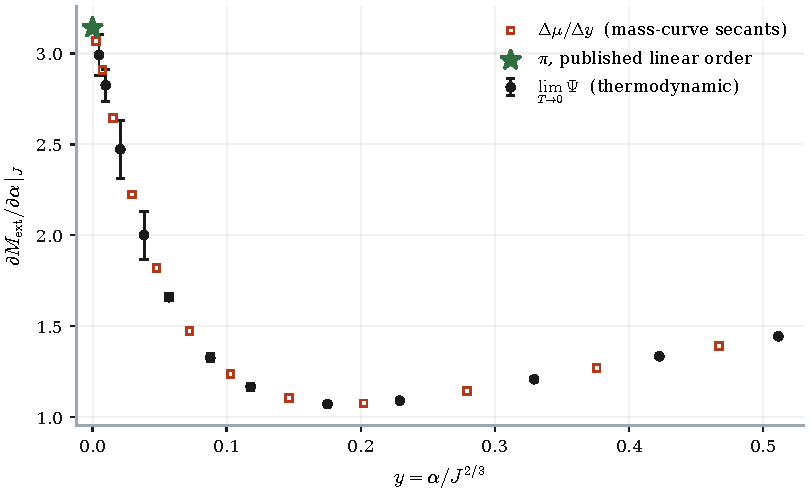
\includegraphics[width=.72\textwidth]{figures/fig-shift.pdf}
\captionof{figure}{Extremal potential against reduced coupling. Circles are extrapolations of $\Psi$; bars indicate fit sensitivity. Squares are secant slopes of $\mu(y)$, which share data with the potential. The star marks the published perturbative value $\pi$.}
\label{fig:shift}
\end{center}

The slope remains positive: it falls from $\pi$ to a lowest sampled value of $1.07$ near $y=0.175$, then rises to $1.44$ at $y=0.511$. The mass increases by about $31\%$. The minimum between points is only bracketed approximately by $0.118<y<0.229$; suppression of the slope does not imply the same suppression of the accumulated mass change.

\begin{center}
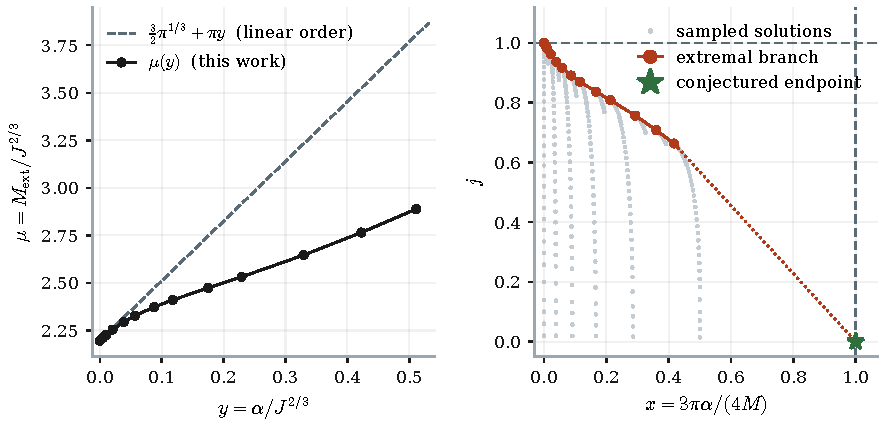
\includegraphics[width=\textwidth]{figures/fig-massext.pdf}
\captionof{figure}{Left: reduced extremal mass against $y$, compared with the first-order prediction. Right: the same branch in $x=3\pi\alpha/(4M)$ and $j=\sqrt{27\pi/8}\,J/M^{3/2}$; grey points are non-extremal states. The star is a conjectured endpoint, and the dotted segment is not computed. All extremal points are extrapolations to $T=0$.}
\label{fig:massext}
\end{center}

\newpage
\section*{5. Revisions, reproducibility, and open questions}
The presentation was audited alongside the calculation. A LaTeX source that failed to compile and left an outdated PDF was corrected, and the maximum cumulative discrepancy of an integral was distinguished from its discrepancy at the end of the interval. Sensitivity budgets, extrapolation plots, Smarr checks, and a more precise discussion of novelty were added. The manuscript's numbers and figures are generated from saved results; commands, versions, and hashes trace their provenance, with documented exceptions.

A subsequent study traversed the 13 couplings at base resolutions $48$ and $56$, with three additional control runs at $64$. Across the 26 resolution runs, the largest recorded change in $\Psi_\ext$ was $6.89\times10^{-5}$, below the corresponding fit sensitivity. This provides a useful check, but not a proof of continuum convergence: many cold states were ultimately refined to $96$ nodes in both sequences, the temperature windows could change, and the numerical environment differed from production. Controls showed that changing the linear algebra stack also changes the adaptive trajectories.

The curvature integral revealed another concrete limitation: increasing the number of nodes indefinitely worsens the result through cancellations in the asymptotic region. The later literature verification recorded 47 checked entries and 11 used without reproduction. That inventory does not amount to checking every claim or successfully running the entire test suite. Closed-form references and general formalisms are distinguished from rederived identities and the project's own numerical results.

Negative results were preserved. The computed ergosurface radius is $1.102101$, against the approximate published value $1.104$ in the case compared; the discrepancy remains open. Failed continuations and provenance exceptions are also retained. Agreement of profiles should not be confused with a full reproduction of a published figure: the required external image is not part of the distribution and was neither obtained again nor reproduced here.

The final scope is a measurement in classical Einstein--Gauss--Bonnet gravity, for one family over a finite interval. A direct extremal construction within this calculation, stronger control of the cold limit, independent global validation, and studies of stability or other branches remain outstanding. The asymptotic behaviour of the slope at arbitrary coupling was not determined. Nor was a universal effective-theory prediction computed: retaining high powers of $\alpha$ in this action does not include the other operators that could contribute in a derivative expansion.

\smallskip
\noindent\textit{About this summary.} This account synthesises archived derivations and measurements; no new production runs were performed. Its checks are limited to the algebraic and documentary consistency recorded in the vault's run receipt and the compilation of these five pages. The three figures are included unchanged from the manuscript; their data were not regenerated.

\vspace{-3pt}
\begin{thebibliography}{9}\small\setlength{\itemsep}{0pt}\setlength{\parskip}{0pt}
\bibitem{er} R. Emparan and H. S. Reall, \textit{Black Holes in Higher Dimensions}, \arxiv{0801.3471}.
\bibitem{gp} G. Goon and R. Penco, \textit{A Universal Relation Between Corrections to Entropy and Extremality}, \arxiv{1909.05254}.
\bibitem{h} G. T. Horowitz et al., \textit{Extremal Kerr black holes as amplifiers of new physics}, \arxiv{2303.07358}.
\bibitem{dsw} Ó. J. C. Dias, J. E. Santos and B. Way, \textit{Numerical Methods for Finding Stationary Gravitational Solutions}, \arxiv{1510.02804}.
\bibitem{egb} Y. Brihaye et al., \arxiv{1010.0860}; B. Kleihaus, J. Kunz and E. Radu, \arxiv{2303.12471}.
\bibitem{pert} L. Ma, Y.-Z. Li and H. Lü, \arxiv{2009.00015}.
\end{thebibliography}
\end{document}
